\chapter{پیاده‌سازی سیستم}

در این قسمت نحوه‌ی اجرای پروژه را بطور کامل توضیح خواهیم داد. در هر قسمت ساختار فایل‌ها، نحوه‌ی پیاده‌سازی و چالش‌هایی که با آن مواجه بودیم به‌همراه نحوه‌ی حل آنها را توضیح خواهیم داد.

\section{معماری کلی سیستم}

برای درک بهتر این پروژه، نمایی کلی از سیستم و نحوه عملکرد آن را همانطور که در \cref{fig:system_overview} نشان داده شده است، ارائه خواهیم داد. این پروژه در چندین محل صنعتی مستقر خواهد شد. در هر کارخانه چندین میکروکنترلر آردوینو، با یک سنسور لرزش و یک فرستنده گیرنده زیگبی متصل، روی هر قطعه از تجهیزات نصب شده است. داده‌ها در زمان‌های برنامه‌ریزی‌شده حس می‌شوند و سپس به دروازه‌ای در کارخانه ارسال می‌شوند. دروازه اطلاعاتی را که از فرستنده‌گیرنده‌های زیگبی می‌آید را جمع‌آوری می‌کند تا زمانی که به یک آستانه‌ی از پیش تعریف‌شده برسد. سپس دروازه با سرور مرکزی احراز هویت می‌شود و سپس داده‌های جمع‌آوری‌شده را با پروتکل \lr{HTTP} به سرور ارسال می‌کند. در سرور مراحل پیش‌پردازش لازم انجام می‌شود و سپس داده‌ها در پایگاه داده‌ی سری زمانی ذخیره می‌شوند. سپس مدل یادگیری ماشین با داده‌های قبلی و جدید اجرا می‌شود تا پیش‌بینی دقیق‌تری درباره طول عمر مفید باقیمانده تجهیزات به ما ارائه دهد. در صورت درخواست، تمام داده‌های تحلیلی و پیشبینی‌ها از طریق داشبورد مدیریت قابل‌دسترسی است. متخصصان می‌توانند از این داده‌ها برای برنامه‌ریزی زمان نگهداری مناسب استفاده کنند.

\begin{figure}[!h]
\centering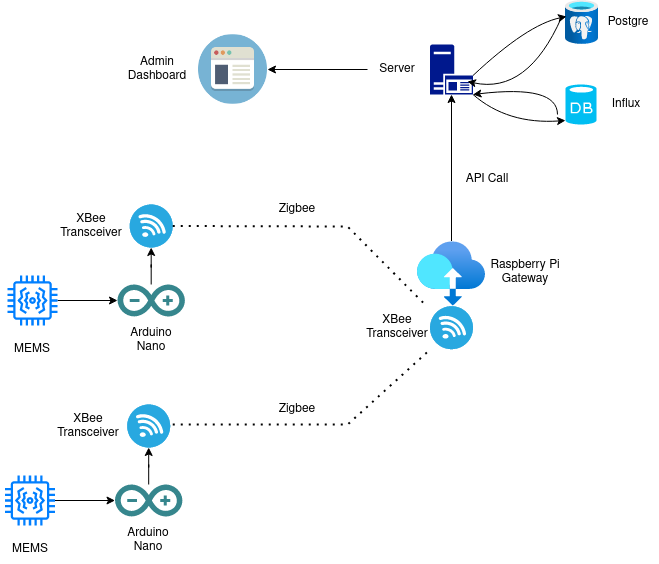
\includegraphics[scale=.6]{system_overview.png}
\caption{نمای کلی سیستم}\label{fig:system_overview}
\end{figure}